\documentclass{article}
\usepackage{amsmath}
\usepackage[]{algorithm2e}
\usepackage{float}
\usepackage{url}
\usepackage{graphicx}


\begin{document}
\title{\textbf{FYS4150/FYS3150 - Project 3}}
\author{Ingvild Bergsbak, Oliver Hebnes and Erlend Ousdal}
\date{October 24, 2018}




\maketitle
\begin{figure}[H]
  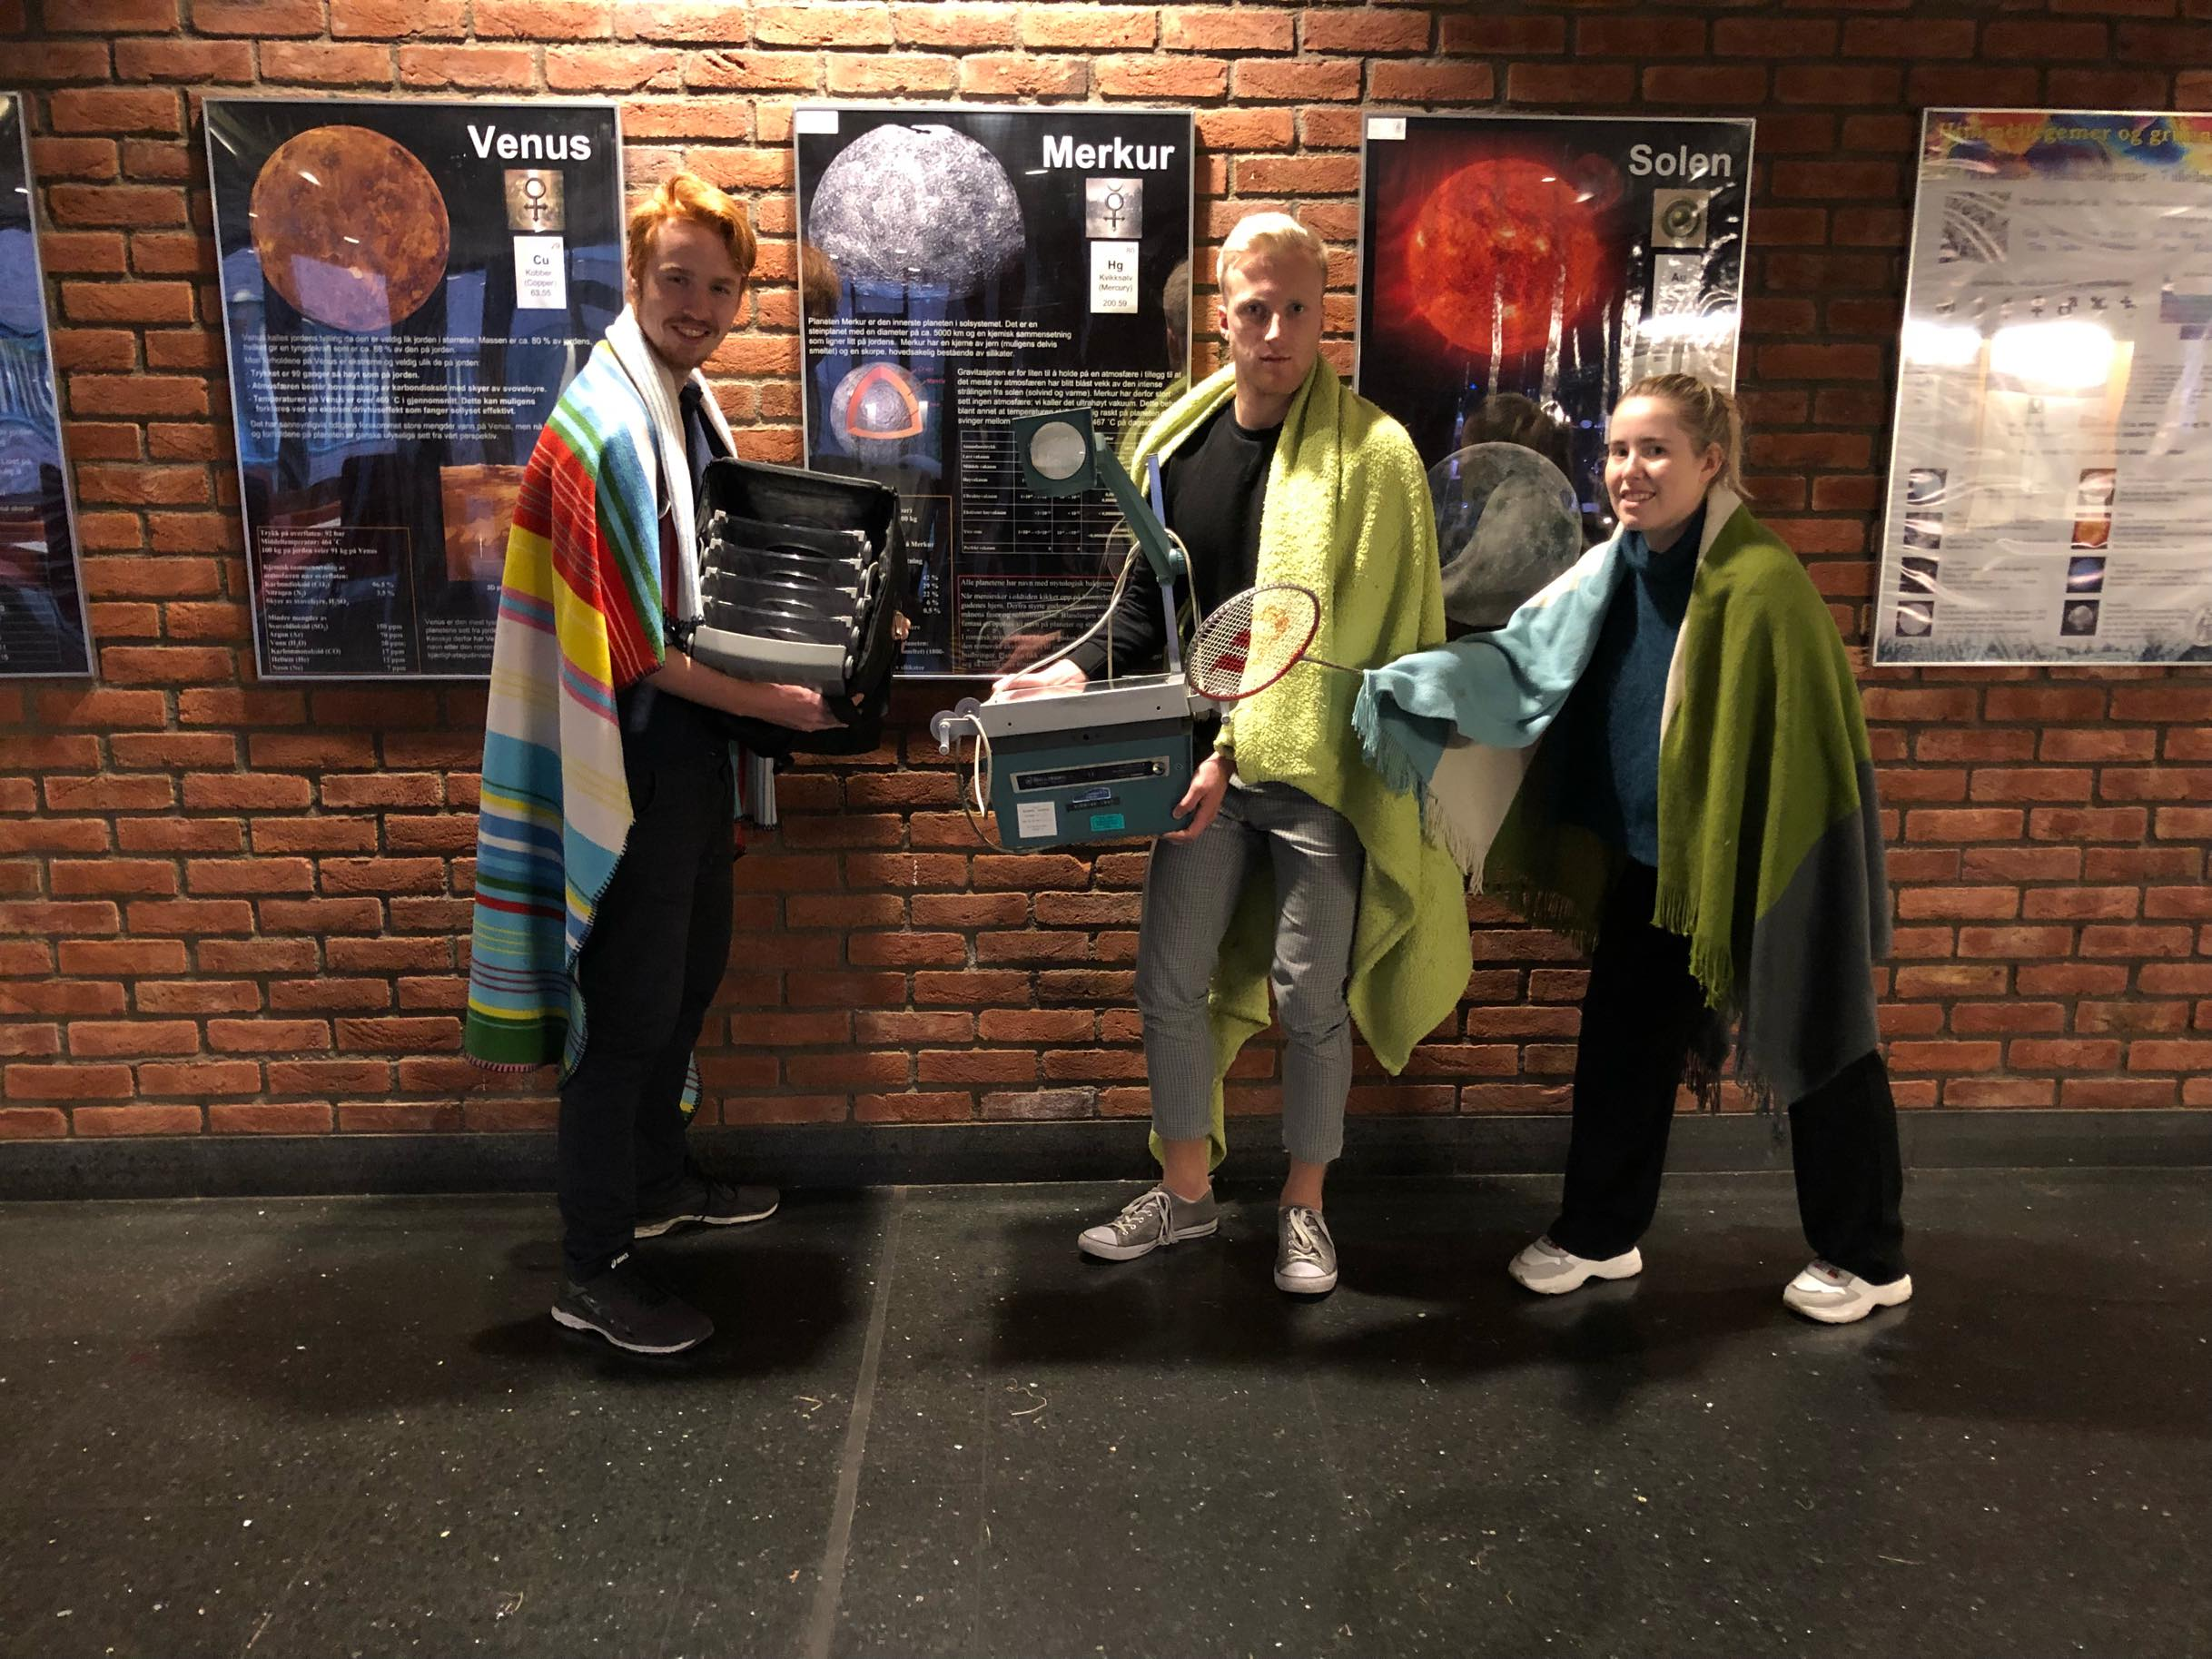
\includegraphics[scale=0.15]{plots/group_pic.jpg}
  \label{}
  \centering
\end{figure}

<<<<<<< HEAD
\newpage
\section{Abstract}
In this project we look at the solar system to compare two different ways to solve differential equations numerically, the Euler and Verlet methods. We found that the Verlet method was more precise than Euler because Verlet conserves the energy. We used object orientation for the planets to make it easy to expand the solar system, and we were able to add and subtract planets and other extra terrestrial objects very easily. We used NASA's webpage \cite{NASA} for the initial conditions. Further on we found that fixing the sun as the center of mass in the solar system is a very good approximation, because if not it would be orbiting within its own radius. As a treat at the end, the perihelion precession of Mercury, when all classical effects were subtracted, was confirmed to be 43 arcseconds as Einstein predicted.

=======
\begin{abstract}
In this project we look at the solar system to compare two different ways to solve differential equations numerically, the Euler and Verlet methods. We found that the Verlet method was more precise than Euler because Verlet conserves the energy. We used object orientation for the planets to make it easy to expand the solar system, and we were able to add and subtract planets and other extra terrestrial objects very easily. We used NASA's webpage \cite{NASA} for the initial conditions. We used the values from October 5, 2018.
\end{abstract}
>>>>>>> eda6fbb085af8865ad248beb2cc4cc921e0a1472

\section{Introduction}
Differential equations are an important part of most fields within physics, and consequently being able to solve them efficiently is an advantage. One of the most basic methods to solve differential equations numerically is the Euler method, and we will be using that and the slightly more advanced Verlet method to model the solar system. The planets of the solar system is a classical differential equation where the gravitational forces give a very good model for the orbits of all the planets. We will use the model to look at the strengths of the different methods.


\section{Theoretical Models and Technicalities}

\subsection{The Euler and Verlet Algorithms}

For a circular orbit around the sun, the force between the sun the the Earth is given by

$$F_G=\frac{M_Ev^2}{r}=\frac{GM_{\odot}M_E}{r^2}$$

where $M_E$ is the mass of Earth and $M_{\odot}$ is the mass of the Sun, and we have that

$$v^2r=GM_{\odot}=\frac{4\pi^2\mathrm{AU}^3}{\mathrm{yr}^2}$$

We use the average distance from the sun to the Earth, AU, as the standard length unit in this project, and for one orbit (the distance $2\pi$ AU) Earth uses one year. We insert AU $=1$ and yr $=1$ and get

$$F_G=\frac{4\pi^2\mathrm{AU}^3M_E}{r^2\mathrm{yr}^2}=\frac{4\pi^2M_E}{r^2}$$


Now we need to decompose the force. To do so we use the fact that $\sin \theta=\frac{r_y}{r}$, $\cos \theta=\frac{r_x}{r}$ and $\sin\phi=\frac{r_z}{r}$, and we get

$$F_{G,x}=\frac{4\pi^2M_E}{r^3}r_x$$
$$F_{G,y}=\frac{4\pi^2M_E}{r^3}r_y$$
$$F_{G,z}=\frac{4\pi^2M_E}{r^3}r_z$$

where $r=\sqrt{r_x^2+r_y^2+r_z^2}$.

Newton's second law gives

$$r_x''=a_x=\frac{F_G}{M_E}=\frac{4\pi^2M_E}{r^3M_E}r_x=\frac{4\pi^2}{r^3}r_x$$
$$r_y''=a_y=\frac{F_G}{M_E}=\frac{4\pi^2M_E}{r^3M_E}r_y=\frac{4\pi^2}{r^3}r_y$$
$$r_z''=a_z=\frac{F_G}{M_E}=\frac{4\pi^2M_E}{r^3M_E}r_z=\frac{4\pi^2}{r^3}r_z$$

\vskip0.5cm
The Euler method generally reads
\vskip0.5cm
\begin{algorithm}[H]
  \For{i=1,n}{
  $x_i=x_{i-1}+h\cdot x_{i-1}'$
  }
\end{algorithm}
\vskip0.5cm

where $h$ is the step size.

In our case we need to calculate both the position and velocity from the acceleration, which is given by the force. This gives us the following algorithm for the $x$ direction

\vskip0.5cm
\begin{algorithm}[H]
  \For{i=1,n}{
$v_{x,i}=v_{x,i-1}-h\frac{4\pi^2}{r^3}r_{x,i-1}$\\
$r_{x,i}=r_{x,i-1}+hv_{x,i-1}$
  }
\end{algorithm}
\vskip0.5cm
The acceleration becomes negative because of the directionality.

The algorithm for $y$ and $z$ direction is identical to the $x$ direction except $x$ is substituted by $y$ and $z$.

\vskip0.7cm
The general velocity Verlet method is given by

\vskip0.5cm
\begin{algorithm}[H]
  \For{i=1,n}{
$x_i=x_{i-1}+hx_{i-1}'+\frac{h^2}{2}x_{i-1}''$\\
$x_i'=x_{i-1}'+\frac{h}{2}(x_{i}''+x_{i-1}'')$
  }
\end{algorithm}
\vskip0.5cm

With our values we get the following algorithm

\begin{equation*}
\begin{split}
a_{x,i-1}=\frac{4\pi^2}{r_{i-1}^3}r_{x,i-1}\\
r_{x,i}=r_{x,i-1}+hv_{x,i-1}+\frac{h^2}{2}a_{x,i-1}\\
a_{x,i}=\frac{4\pi^2}{r_i^3}r_{x,i}\\
v_{x,i}=v_{x,i-1}+\frac{h}{2}(a_{x,i}+a_{x,i-1})
\end{split}
\end{equation*}

\vskip0.5cm
\begin{algorithm}[H]
  \For{i=1,n}{
$a_{x,i-1}=\frac{4\pi^2}{r_{i-1}^3}r_{x,i-1}$\\
$r_{x,i}=r_{x,i-1}+hv_{x,i-1}+\frac{h^2}{2}a_{x,i-1}$\\
$a_{x,i}=\frac{4\pi^2}{r_i^3}r_{x,i}$\\
$v_{x,i}=v_{x,i-1}+\frac{h}{2}(a_{x,i}+a_{x,i-1})$
  }
\end{algorithm}
\vskip0.5cm


Again, we only write the algorithm for the $x$ direction, but the $y$ and $z$ direction is completely analogous.


\subsection{The Three-Body System}

The next step towards modeling the whole solar system is to add one planet, Jupiter, to our system. The force between Earth and Jupiter is given by
$$F_{EJ}=\frac{GM_JM_E}{r_{EJ}^2}$$

where $M_J$ is the mass of Jupiter and $r_{EJ}$ is the distance between Earth and Jupiter. Decomposing the forces gives

$$F_{EJ,x}=\frac{GM_JM_E}{r_{EJ}^3}(r_{J,x}-r_{E,x})$$
$$F_{EJ,y}=\frac{GM_JM_E}{r_{EJ}^3}(r_{J,y}-r_{E,y})$$
$$F_{EJ,z}=\frac{GM_JM_E}{r_{EJ}^3}(r_{J,z}-r_{E,z})$$

The total force that works on Earth becomes

$$F_{E,x}=F_{G,x}+F_{EJ,x}=\frac{4\pi^2M_E}{r^3}r_x+\frac{GM_JM_E}{r_{EJ}^3}(r_{J,x}-r_{E,x})$$
$$F_{E,y}=F_{G,y}+F_{EJ,y}=\frac{4\pi^2M_E}{r^3}r_y+\frac{GM_JM_E}{r_{EJ}^3}(r_{J,y}-r_{E,y})$$
$$F_{E,z}=F_{G,z}+F_{EJ,z}=\frac{4\pi^2M_E}{r^3}r_z+\frac{GM_JM_E}{r_{EJ}^3}(r_{J,z}-r_{E,z})$$

and similarly for Jupiter

$$F_{J,x}=F_{GJ,x}+F_{JE,x}=\frac{4\pi^2M_J}{r^3}r_x+\frac{GM_JM_E}{r_{JE}^3}(r_{E,x}-r_{J,x})$$
$$F_{J,y}=F_{GJ,y}+F_{JE,y}=\frac{4\pi^2M_J}{r^3}r_y+\frac{GM_JM_E}{r_{JE}^3}(r_{E,y}-r_{J,y})$$
$$F_{J,z}=F_{GJ,z}+F_{JE,z}=\frac{4\pi^2M_J}{r^3}r_z+\frac{GM_JM_E}{r_{JE}^3}(r_{E,z}-r_{J,z})$$

Now that we have all the forces that work on each object, we use the same algorithm as before to calculate the position and velocity of Earth and Jupiter.

\subsection{Object Orientation and the Rest of the Solar System}
The next step now is to implement more planets. To do so we choose to introduce a new class called "Planets". It is defined as an object that includes the different parameters of the planet that we use; mass, distance from the sun and initial position and velocity. By introducing a function that calculates the forces that work between all the planets, we are now able to add any celestial body in our solar system to our model. The forces between the planets are calculated in the same way as the force between Earth and Jupiter in the previous section, and by adding all the forces we get the total force on each planet. Another function calculates the position and velocity using the Verlet method and the force (or the acceleration).

\subsection{Perihelion Precision of Mercury}
The perihelion is the point on Mercury's orbit where the distance between Mercury and the Sun is shortest. On a perfect elliptical the perihelion will stay constant, but when taking the relativistic correction into account the point will gradually shift, although the distance remains constant. The given value for the rotation is 43 arc seconds per 100 years, which corresponds to about $0.0119^{\circ}$ or 0.0002085 radians. To implement the relativstic correction, we change the gravitational force to

$$F_G=\frac{GM_{\mathrm{Sun}}M_{\mathrm{Mercury}}}{r^2}\bigg( 1+\frac{3l^2}{r^2c^2}\bigg)$$

where $l$ is the angular momentum and $c$ is the speed of light in vacuum.


\section{Results and Discussion}

\subsection{Earth-sun system}
It was found that the initial velocity that gives a circular orbit was $2\pi$, as given in \ref{jordensbane}.
\begin{figure}[H]
  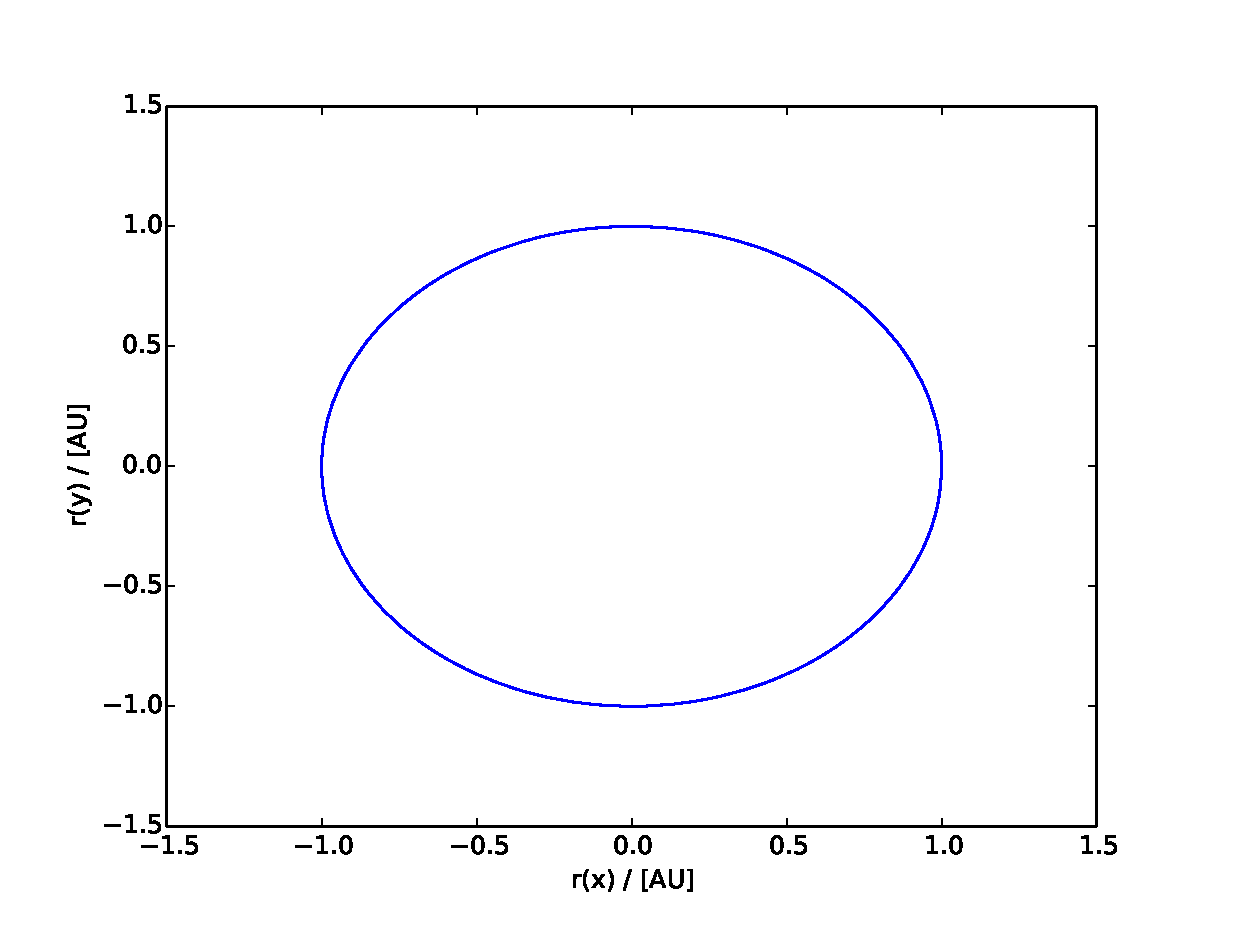
\includegraphics[scale=0.6]{plots/3c_jordensbane_verlet_n10e6.eps}
  \caption{The Earth in a circular orbit around the origin (the sun) with intial velocity $2\pi$ in positive vertical direction. This is done by using Veilet's algorithm with $10^6$ integration points.}
  \label{jordensbane}
\end{figure}

\begin{table}[H]
    \centering
    \begin{tabular}{|l|c|c|c|r|}
    \hline
     $n$ & Verlet error / AU & Euler error & Time Verlet / [s] & Time Euler / [s]\\
     \hline
      $10^5$  & $3.1\cdot10^{-14}$  & $7.3\cdot10^{-2}$ & $ 2.0 (30) \cdot 10^{-2}$ & $ 2.1 (3) \cdot 10^{-2}$\\
      $10^6$  & $2.1\cdot10^{-13}$  & $7.9\cdot10^{-3}$ & $ 9.22 (27) \cdot 10^{-2}$ & $ 5.40 (40)\cdot 10^{-2}$\\
      $10^7$  & $4.3\cdot10^{-14}$  & $7.90\cdot10^{-4}$ & $ 7.3 (29) \cdot 10^{-1}$ & $ 4.7 (36) \cdot 10^{-1}$\\
      $10^8$  & $2.2\cdot10^{-12}$  & $7.90\cdot10^{-5}$ & $ 7.20 (35) \cdot 10^{0}$ & $ 4.2 (45) \cdot 10^{0}$\\
      $10^9$  & $1.4\cdot10^{-11}$  & $7.90\cdot10^{-6}$ & $ 7.3 (35) \cdot 10^{1}$ & $ 4.0 (45) \cdot 10^{1}$\\
      \hline
    \end{tabular}
    \caption{Testing the stability and time used for Euler's algorithm and Verlet's algorithm.}
    \label{stability}
\end{table}

When comparing Euler's forward algorithm with Verlet's algorithm, it is clear that Verlet is a very accurate method compared to Euler's forward algorithm. The error for Euler scales as $\frac{1}{N}$, while the error for Verlet's method is so small that the machine precision is having trouble managing the numbers. Even if Verlet uses a bit more time than Euler (naturally, because Euler's method scales as 12n flops while Verlet's method scales like 18n flops), we see that it is a small sacrifice for a much greater accuracy for our solar system.

We implemented a test in our program that checked if the length of the position vector stayed within a known tolerance, because this should be the case if the potential energy is conserved.

This is also true with the kinetic energy, but this time we tested if the length of the velocity-vector stayed constant. We found results that correlate with table \ref{stability}; if the number of integration points increase, the tolerance can be decreased. The precision for Verlet is very good, which means we could use a very small tolerance ($\epsilon = 10^{-14}$). For Euler's method - not so much ($\epsilon = 10^{-2}$), which means we can draw the conclusion that Verlet's method conserves the energy while Euler's method does not.

If both the kinetic and potential energy is conserved, so will the angular momentum. This is because angular momentum is given by the formula $\vec{L}=\vec{r} \times \vec{p} =m \vec{r} \times \vec{v}$.


Thus we continued with Verlet's method as we further on explored the solar system using his algorithm.

\subsection{Escape Velocity}
The exact value for the escape velocity can be calculated from the equation
$$v_{\mathrm{escape}}=\sqrt{\frac{2GM_{\odot}}{r}}$$
Inserting for the gravitational constant, sun mass and assuming the distance $r$ is 1 AU, we get an exact answer for the escape velocity, $v_{\mathrm{escape}}\approx 8.861$ AU/yr. We find with our model by trial and error that Earth escapes the Sun with a velocity of about $8.88$ AU/yr, which is fairly close to the exact value.

By changing the gravitational force to
\begin{align*}
  F_G = \frac{GM_{\odot}M_{Earth}}{r^{\beta}}
\end{align*}
where $\beta$ is approaching the number $3$, one can observe a change in circular orbit velocity, potential energy and escape velocity. The circular orbit velocity results in
\begin{align*}
  v_{circular}=\sqrt{\frac{GM_{\odot}}{r^{\beta-1}}}
\end{align*}

Integrating the force results in the potential as
\begin{align*}
  U = \int_0^r \vec{F} d\vec{r} =  \frac{GM_{\odot}M_{Earth}}{(\beta-1)} \frac{1}{r^{\beta-1}}
\end{align*}
If we set $\beta$ as $3$, we find the escape velocity as
\begin{align*}
  v_{escape} = \sqrt{\frac{GM_{\odot}}{2}} \frac{1}{r}
\end{align*}
Oh'man this system is unstable, because
\begin{align*}
  v_{escape} = \frac{1}{\sqrt{2}}\cdot v_{circular}
\end{align*}
which tells us that whatever initial velocity the earth starts with the system would go insanely bananas (unstabile). This is also accurate according to figures \ref{beta25} and \ref{beta35}.

\begin{figure}[H]
  \includegraphics[scale=0.6]{plots/b35.eps}
  \caption{Earth-sun system with Beta $= \beta - 1 = 2.5$, where the earth is having a tendency to not move in a closed circular orbit}
  \label{beta25}
\end{figure}

\begin{figure}[H]
  \includegraphics[scale=0.6]{plots/b40.eps}
  \caption{Earth-sun system with Beta $= \beta - 1 = 3$, where the earth cleary is not moving in a closed circular orbit}
  \label{beta35}
\end{figure}

\subsection{The three body problem}
When increasing the mass of Jupiter in a system with the Earth in a circular orbit around around a fixed center of mass (the Sun), one finds that the earth will also orbit around Jupiter when the mass gets comparable (and bigger).

\begin{figure}[H]
  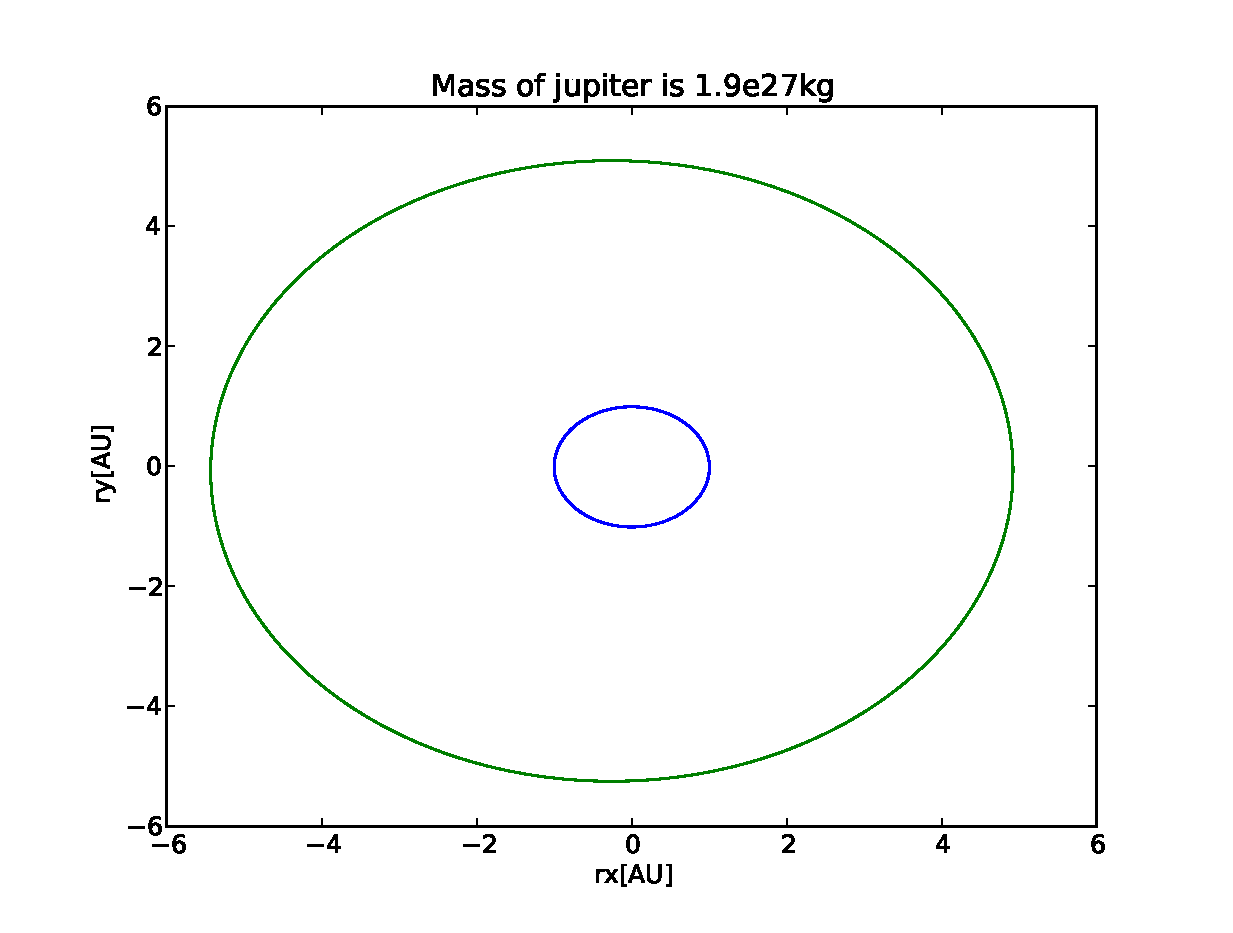
\includegraphics[scale=0.5]{plots/Mass1.eps}
  \caption{The sun (as the center of mass), Jupiter (with its original mass) and the earth in the solar system. Number of time steps is ten million}
  \label{jupitermass1}
\end{figure}

\begin{table}[H]
    \centering
    \begin{tabular}{|l|c|r|}
    \hline
     $n$ & Max difference in angular momentum in ${\textnormal{ AU}}^2\textnormal{/yr}$ & Time Verlet / [s] \\
     \hline
      $10^4$  & $4.91\cdot10^{-4}$  & $3.0\cdot10^{-2}$\\
      $10^5$  & $4.91\cdot10^{-4}$  & $2.0\cdot10^{-1}$ \\
      $10^6$  & $4.91\cdot10^{-4}$  & $1.71\cdot10^{0}$\\
      $10^7$  & $4.91\cdot10^{-4}$  & $2.1\cdot10^{1}$\\
      $10^8$  & $4.91\cdot10^{-4}$  & $1.56\cdot10^{2}$\\
      \hline
    \end{tabular}
    \caption{Test of the stability of the three-body problem with Jupiter having its original mass.}
    \label{Three-body-problem}
\end{table}

The stability of figure \ref{jupitermass1} is tested as a function of position and velocity in table \ref{Three-body-problem}. The stability is pretty neat when Jupiter is at its original mass, resulting in the same difference in angular momentum for each simulation with different time steps.


\begin{figure}[H]
  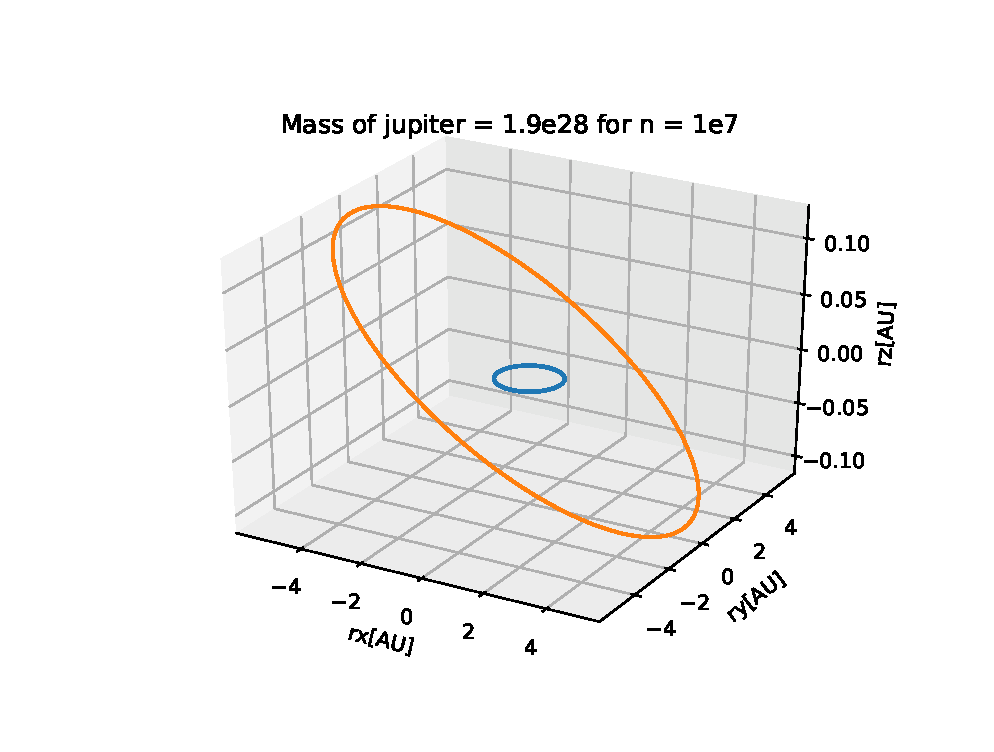
\includegraphics[scale=0.5]{plots/Mass10.eps}
  \caption{The sun (as the center of mass), Jupiter (with ten times its original mass) and the Earth in the solar system. Number of timesteps is ten million.}
  \label{jupitermass10}
\end{figure}

\begin{figure}[H]
  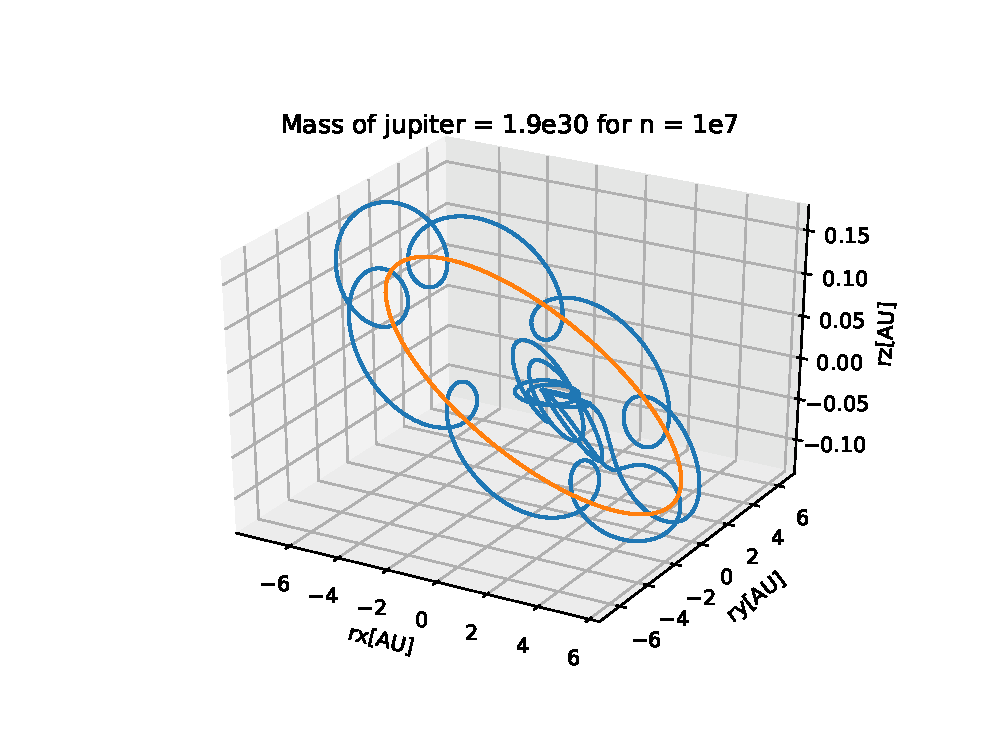
\includegraphics[scale=0.6]{plots/Mass1000.eps}
  \caption{The sun (as the center of mass), Jupiter (with a thousand times its original mass) and the Earth in the solar system. Number of timesteps is one hundred billion for better precision.}
  \label{jupitermass1000}
\end{figure}

From figure \ref{jupitermass1000} the earth will move in an epicycle \cite{epicycle}, which means Jupiter will alter the Earth's motion around the Sun and make it orbit around Jupiter as well.



\begin{table}[H]
    \centering
    \begin{tabular}{|l|c|r|}
    \hline
     $n$ & Max difference in angular momentum in ${\textnormal{ AU}}^2\textnormal{/yr}$ & Time Verlet / [s] \\
     \hline
      $10^4$  & $1.0\cdot10^{3}$  & $2.7\cdot10^{-2}$\\
      $10^5$  & $7.0\cdot10^{1}$  & $1.9\cdot10^{-1}$ \\
      $10^6$  & $6.7\cdot10^{1}$  & $1.7\cdot10^{0}$\\
      $10^7$  & $6.7\cdot10^{1}$  & $1.6\cdot10^{1}$\\
      $10^8$  & $6.7\cdot10^{1}$  & $1.6\cdot10^{2}$\\
      \hline
    \end{tabular}
    \caption{Test of the stability of the three-body problem with Jupiter having a thousand times its original mass}
    \label{Three-body-problem-jupiter}
\end{table}

For the case when Jupiter has ten thousand times its own mass, the difference in angular momentum converges towards $67 {\textnormal{ AU}}^2\textnormal{/yr}$.


\subsection{Final model of all planets of the solar system}
When adding all planets in the solar system (including Pluto), and in addition giving the sun a initial velocity while not being in the center of mass, results in figure \ref{solarsystem}. When comparing this with to the sun fixed at the center of mass at figure \ref{fixedsolarsystem}, it shows that even though the sun is not at our fixed position of center of mass, the deviation the sun has from the origin is very low. This means that the mass of the sun is of a tremendous character compared to the other planets of the solar system.

\begin{figure}[H]
  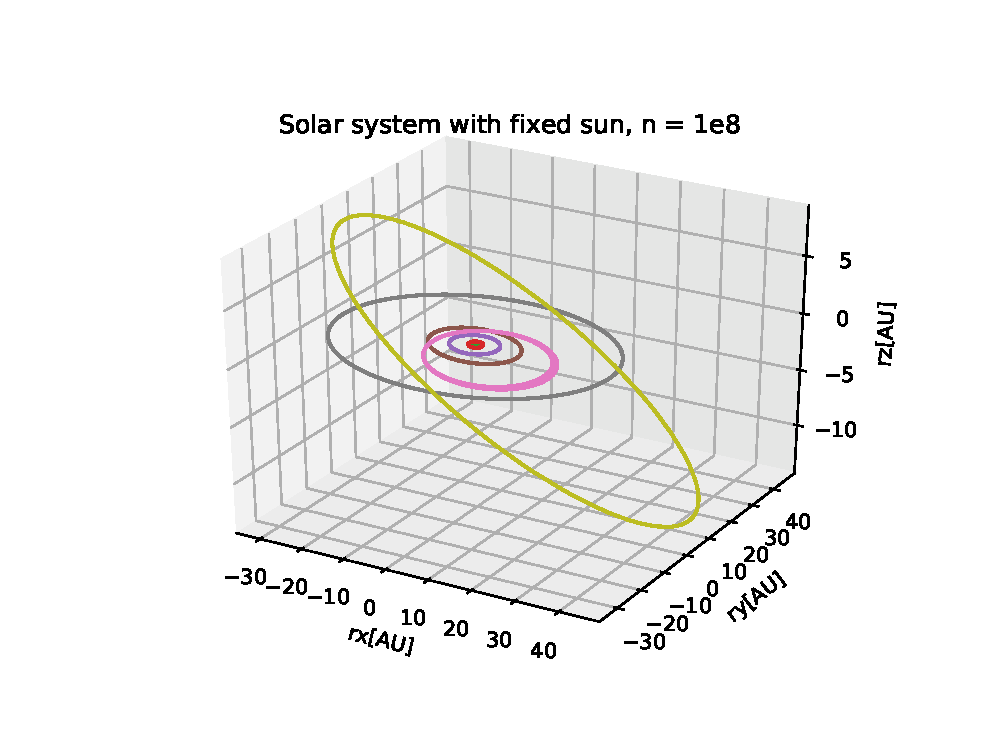
\includegraphics[scale=0.7]{plots/FixedSolarSystem.eps}
  \caption{The solar system with the sun fixed at the center of mass.}
  \label{fixedsolarsystem}
\end{figure}

\begin{figure}
  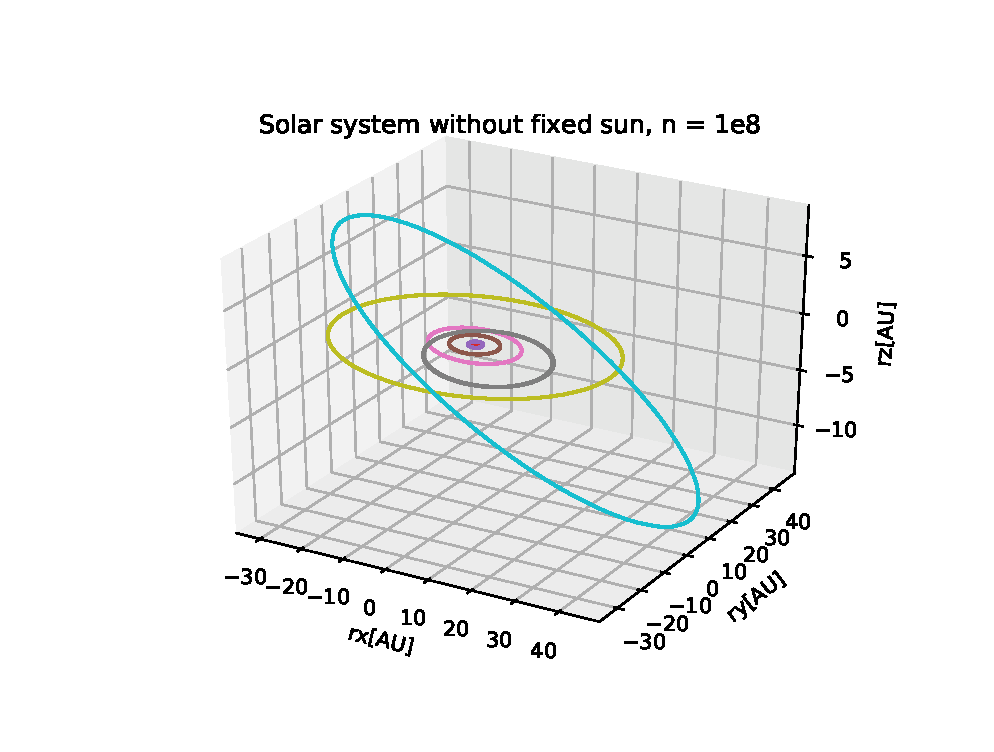
\includegraphics[scale=0.7]{plots/SolarSystem.eps}
  \caption{The solar system without the sun at the center of mass.}
  \label{solarsystem}
\end{figure}


\subsection{Perihelion Precision}


\vskip0.5cm
As for the question about whether Mercury's perihelion precision can be described by the general theory of relativity, the answer is yes. When Einstein developed his theory, he used the rotation of Mercury's elliptical orbit as an argument for why his theory was so strong. \cite{wiki_rel}



\section{Conclusion}

We have have found that the Verlet method shows superior stability over Euler, and even though Euler is faster, the numerical precision of Verlet proves a huge advantage when dealing with problems of this magnitude; Rome wasn't built in a day, and neither was our solar system. The art of object oriented programming, OOP for short, though only at our apprentice level, shows great potential for future computational physics challenges. It has been exciting to be able to model our solar system as accurately as we have, using nothing more than simple ordinary differential equations. 

As an evaluation of our work throughout the project, we should have been better at saving our results as we produced them instead of having to go back to reproduce them before delivery.


\section{Appendix}
Link to the GitHub repository:\\

https://github.com/ohebbi/compphys.git

\begin{thebibliography}{}
\bibitem{NASA}
<<<<<<< HEAD
NASA Jet Propulsion Laboratory, California Institute of Technology, downloaded 05.10.18\\
=======
California Institute of Technology, \textit{NASA Jet Propulsion Laboratory}, downloaded 05.10.18\\
>>>>>>> eda6fbb085af8865ad248beb2cc4cc921e0a1472
\url{http://ssd.jpl.nasa.gov/horizons.cgi# top}
\bibitem{wiki_rel}
Wikipedia, \textit{General Relativity}, downloaded 24.10.18\\
\url{https://en.wikipedia.org/wiki/General_relativity}
\bibitem{epicycle}
Store Norske leksikon, \textit{Episykel}, downloaded 24.10.18\\
\end{thebibliography}



\end{document}
